% arara: pdflatex: { synctex: yes }
% arara: makeindex: { style: ctuthesis }
% arara: bibtex

% The class takes all the key=value arguments that \ctusetup does,
% and a couple more: draft and oneside
\documentclass[twoside]{ctuthesis}
\usepackage{booktabs}
\usepackage{graphicx}
\usepackage{enumitem}
\usepackage{subcaption}

\ctusetup{
%	preprint = \ctuverlog,
%	mainlanguage = english,
	mainlanguage = english,
%	titlelanguage = english,
	otherlanguages = {slovak,czech},
	title-czech = {Vizualizace urbanistických dat},
	title-english = {Urban Data Visualization},
	subtitle-czech = {Zpráva k semestrálnímu projektu},
	subtitle-english = {Semestral Project Report},
	xdoctype = M,
	xfaculty = F3,
	department-czech = {Katedra počítačové grafiky a interakce},
	department-english = {Department of computer graphics and interaction},
	author = {Vojtěch Tomas},
	supervisor = {Ing. David Sedláček, Ph.D.},
%	supervisor-address = {Ústav X, \\ Uliční 5, \\ Praha 99},
%	supervisor-specialist = {John Doe},
%	fieldofstudy-english = {Mathematical Engineering},
%	subfieldofstudy-english = {Mathematical Modelling},
%	fieldofstudy-czech = {Matematcké inženýrství},
%	subfieldofstudy-czech = {Matematické modelování},
	keywords-czech = {slovo, klíč},
	keywords-english = {word, key},
	day = 14,
	month = 1,
	year = 2021,
	specification-file = {ctutest-zadani.pdf},
%	front-specification = true,
%	front-list-of-figures = false,
%	front-list-of-tables = false,
%	monochrome = true,
%	layout-short = true,
}

\ctuprocess

\addto\ctucaptionsczech{%
	\def\supervisorname{Vedoucí}%
	\def\subfieldofstudyname{Studijní program}%
}

\ctutemplateset{maketitle twocolumn default}{
	\begin{twocolumnfrontmatterpage}
		\ctutemplate{twocolumn.thanks}
		\ctutemplate{twocolumn.declaration}
		\ctutemplate{twocolumn.abstract.in.titlelanguage}
		\ctutemplate{twocolumn.abstract.in.secondlanguage}
		\ctutemplate{twocolumn.tableofcontents}
		\ctutemplate{twocolumn.listoffigures}
	\end{twocolumnfrontmatterpage}
}

% Theorem declarations, this is the reasonable default, anybody can do what they wish.
% If you prefer theorems in italics rather than slanted, use \theoremstyle{plainit}
%\theoremstyle{plain}
%\newtheorem{theorem}{Theorem}[chapter]
%\newtheorem{corollary}[theorem]{Corollary}
%\newtheorem{lemma}[theorem]{Lemma}
%\newtheorem{proposition}[theorem]{Proposition}

%\theoremstyle{definition}
%\newtheorem{definition}[theorem]{Definition}
%\newtheorem{example}[theorem]{Example}
%\newtheorem{conjecture}[theorem]{Conjecture}

%\theoremstyle{note}
%\newtheorem*{remark*}{Remark}
%\newtheorem{remark}[theorem]{Remark}

%\setlength{\parskip}{2ex plus 0.2ex minus 0.2ex}
\widowpenalty10000
\clubpenalty10000

% Abstract in Czech
\begin{abstract-czech}
TODO
\end{abstract-czech}

% Abstract in English
\begin{abstract-english}
TODO
\end{abstract-english}

% Acknowledgements / Podekovani
\begin{thanks}
Děkuji ČVUT, že mi je tak dobrou \emph{alma mater}.
\end{thanks}

% Declaration / Prohlaseni
\begin{declaration}
Prohlašuji, že jsem předloženou práci vypracoval samostatně, a že jsem uvedl veškerou použitou literaturu.

V Praze, \ctufield{day}.~\monthinlanguage{title}~\ctufield{year}
\end{declaration}

\begin{document}

\maketitle


\chapter{Introduction}
In recent years, cities have become a huge source of various data. The urban data usually includes street layouts, public transport information, layouts of the power network, noise maps, socio-economic maps, etc. The first natural question is, why should we care about the urban data? Why do we bother coming up with creative ways to present the data publicly?

All plans and future changes are made and approved based on the models derived from the urban data. As the city develops, people adapt, and newer data is generated. Newer data can help building newer, better models. The city planning process is a loop with city planners on one side and stakeholders together with general public on the other, see ilustration \ref{fig:loop1}.  

\begin{figure}[h]
    \centering
    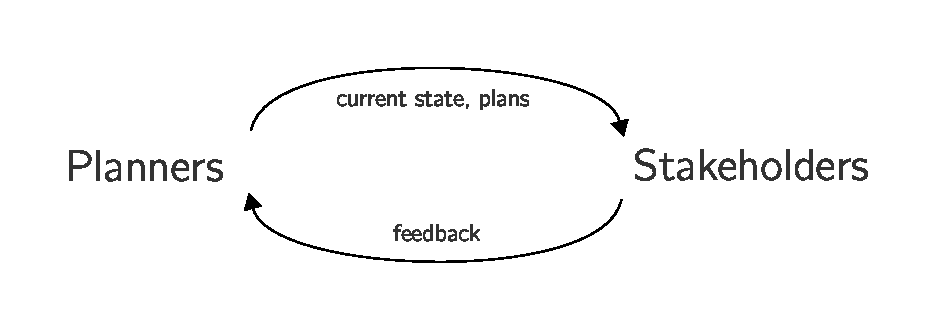
\includegraphics[width=0.7\linewidth]{figures/Loop1.pdf}
    \caption{Basic city planning loop}
    \label{fig:loop1}
\end{figure}

Looking at this loop from the stakeholders' perspective, it is in their best interest to influence the decision-making process in their favour. Similarly, local authorities should strive for more interaction between the city administration and the public. This involves making the urban data publicly available and accessible.

\section{From Data to Visualization}
As of today, the urban data is usually freely accessible in a format that is obscure for the general public. Naturally, to make the data more accessible, it is necessary to visualize it. Local authorities usually make this effort with either one of the following goals: 
\begin{itemize}
    \item to inform the public about the current state,
    \item or present the effects of a future change in the area.
\end{itemize}

Communicating the current state usually requires analysis and simplification of the raw data. There is a wide range of tools for that; however, these tools are usually proprietary, and the outputs are not that engaging. The visualization is rarely customizable; proprietary formats are used throughout the entire pipeline, and it is impossible to combine various types of data.

Communicating the future changes is even more difficult since it is required to inform the public about the current state first. In this context, the interactivity of the presentation can be the key to understanding.

We are presented with several technical challenges. The input data is often in several incompatible formats, and each describes a completely different urban domain. In other words, the datasets are often complementary, and the visualization system has to support their combination. For example, some data use different coordinate systems, or the datasets differ in their dimensionality.

If we want to create a \textit{usefull} visualization, the aforementioned technical obstacles should remain hidden from both the visualization creator and also the audience. In the ideal case, the visualization creator is given absolute freedom. The visualization system does not pose any hard restrictions on what is possible; the creator's imagination is the only limit. This utopistic idea is often contradicted by the requirement of a simple and usable interface. It is appropriate to seek a balance between unlimited possibilities and usability.

Taking into account the viewer's perspective, the goal is to make the visualization immersive enough to captivate, educate, and entertain. The physical setup and software capabilities should not diminish the experience and should avoid posing any virtual barriers between the medium and the audience.

Usually, the visualization is presented in a public space, either in museums or centers specifically equipped for this kind of presentation. While some of these places own the necessary equipment, the production pipeline today is often complicated, and an ad-hoc solution is used. In other cases, the visualization is presented using proprietary software, which is not primarily designed for the general public.

\section{The Goals}
The goal is to develop a modular system, which will streamline the urban data visualization process. The design should focus on the following four factors:
\begin{itemize}
    \item the actual communicated information,
    \item the nature of the available urban data,
    \item the creator's artistic vision,
    \item and the equipment used for the presentation.
\end{itemize}
The tricky part is that probably only one or two of those factors are known in advance --- the urban data and the used equipment can be somewhat standardized. The remaining two factors are usually project-specific; therefore, it is necessary to explore the combination of various data types and enable the freedom of artistic expression. The goal is to build a system for building other systems because of the desired modularity and adjustability --- there is an inherent metaprogramming element.
\chapter{Urban Data}
This chapter aims to describe the nature of urban data --- the sources, classification, and available formats. To some extent the term \textit{urban data} is somewhat simmilar to other buzzwords, such as \textit{big data}. As there is no official definition of the term \textit{urban data}, it is often explaied by giving a list of examples, such as transport data or socio-economic maps. The urban data is a subject of study in several fields, one of which is the Urban Informatics.

\section{Urban Informatics}
In 2011, Forth et al. \cite{foth2011urban} described Urban Informatics as a separate field of study. It focuses on three key aspects --- place, technology, and people in the context of urban environments. The urban environment is described as a \textit{"complex techno-social network; the city only meaningfully exists when a sustained stream of people occupies it"} \cite{foth2011urban}. The authors outline and study four dominant trends: the emergence of ubiquitous computing, the accessibility of real-time information, informed sustainability, and planning based on citizen participation. 

One of the goals of Urban Informatics is to help developing communication channels between local authorities and citizens. Moreover, thanks to the gathered information, the citizens can, directly and indirectly, influence the development of the urban area. The communication channels, as understood by Urban Informatics, are omnidirectional. 

\section{Sources of Urban Data}
This section contains description of three main urban data sources. This clasification is based on the summary presented in \cite{robinson2012street}. The urban data sources include mainly governments and local administrative institutions. Additionaly, the data is gathered and received through devices that are part of the ubicomp device system. The third source of urban data consists of online services, such as social networks. 

\paragraph{Open Data}
The most prominent source of data are governments and local institutions. The data is commonly released in several open formats, which are further described in the section \ref{sec:formats}. This data often includes maps, building layouts, terrain models, technical metadata, public transport data, etc. The formats range from generic CSV or SQLite-based to domain-specific DWG, CityGML, etc.   
The data presented earlier are mainly static; some cities also offer real-time information about weather or public transport vehicle locations. 

\paragraph{Ubicomp} Mark Weiser first introduced Ubiquitous Computing in 1991 \cite{weiser1991computer}. The concept of ubicomp relies on small embedded computers, which communicate together and allow for seamless interaction between users and technology. Accoring to \cite{zheng2011urban}, the ubiquitous information's impact on the city level became the focus of study in a separate field called Urban Computing. In the spirit of ubiquitous computing, there is an emerging field of Participatory Sensing \cite{burke2006participatory}, which enables gathering data from devices of individual users. The design of the participation model focuses on data credibility, security, and privacy protection. One of the applications of Participatory Sensing is the use of the gathered data for urban planning. 

\paragraph{Online services}
Personal data can also be acquired from social networks or mobile phone carriers. Online platforms usually support geotagging, adding geospatial metadata to the content posted online. The content can be easily queried based on the selected location. Alternatively, the citizens' location can be tracked via their mobile phone directly by carriers using the individual base transceiver stations (BTS).  From the perspective of Urban Informatics, the aforementioned data sources enable creating richer urban area models. 

\section{Urban Data Domains}
There is no official classification of the urban data. However, open data portals usually use custom classification schemes, which are either domain or format-based. Based on the available open data catalogues of the cities in 5 Cities Connect\footnote{Prague has been recently invited into the 5CC initiative} group \cite{5CC}, a list of domain classes has been assembled, see table \ref{tab:opendata}. The listed domains are either of significant importance or have appeared across a majority of the reviewed catalogues.  


% Please add the following required packages to your document preamble:
% \usepackage{booktabs}
\begin{table}[]
    \resizebox{0.9\textwidth}{!}{
    \begin{tabular}{@{}lllllll@{}}
    \toprule
    Domain                   & Hamburg & Vienna & Rotterdam & Helsinki & Singapur & Prague \\ \midrule
    Buildings                & x       & x      & x         & x        &          & x      \\
    Population and Work      & x       & x      &           & x        & x        & x      \\
    Technical infrastructure & x       & x      &           & x        & x        & x      \\
    Transport                & x       & x      & x         & x        & x        & x      \\
    Geology                  & x       &        & x         &          &          & x      \\
    Noise maps               &         & x      &           & x        &          & x      \\
    Environment and Nature   & x       & x      & x         & x        & x        & x      \\
    Ortographic maps         & x       & x      & x         & x        & x        & x      \\
    Public services          & x       & x      & x         & x        & x        & x      \\
    Terrain                  &         & x      & x         & x        &          & x      \\
    Air Quality              &         &        & x         & x        & x        & x      \\
    Zoning Plan              &         & x      & x         & x        & x        & x      \\ \bottomrule
    \end{tabular}}
    \caption{Urban data classes availability on open data portals}
    \label{tab:opendata}
\end{table}


\section{File Formats}
\label{sec:formats}
This section describes the file formas used to store various urban data. Some of these file formats are proprietary; however, from the perspective of application development, open formats are more attractive. 

\paragraph{Esri Shapefiles} 
Esri Shapefile \cite{esri1998shapefile} is generally a vector data file format for a geographic information system. A single shapefile consists of several files; the minimal set of files necessary for correct data interpretation is  DBF, SHP, and PRJ file: 

\begin{description}[noitemsep]
    \item[SHP] contains the actual geometry,
    \item[DBF] contains the attributes and indexes,
    \item[PRJ] describes the coordinate reference system.  
\end{description}
In the original specification \cite{esri1998shapefile}, SHX is also a mandatory file. Still, the file only allows to accelerate the queries and is not required for the data to be displayed correctly. The Shapefile format is well documented, and there is a range of existing importers in various languages. 


\paragraph{CityGML and CityJSON}
CityGML \cite{groger2012ogc} is an XML-based file format designed to capture the structure and metadata of 3D city models. The aim of the development is to come up with a standardized and sustainable way of storing urban data. There is a JSON-based version of CityGML - CityJSON \cite{ledoux2019cityjson}. Despite minor differences, these two standards are mostly compatible. From the practical point of view, the CityJSON format is much less verbose and thus easily parsable. Both CityGML and CityJSON are open formats; there are convertors and importers available .

\paragraph{GeoJSON}
Another JSON-based standard is the GeoJSON format. This GeoJSON structure is quite simple; the file can describe a set of primitive geometry objects such as lines, lines, or polygons. Each primitive can have a variable number of properties, which can be completely arbitrary. The GeoJSON file usually describes data such as networks or areas. Compared to CityJSON, GeoJSON is not suitable for representing hierarchies, which usually naturally appear in building geometry and its components. GeoJSON is an open format, it is fairly simple to write an importer for this format, and there are several available, see \cite{cityJSONconvert, cityGMLimport}. 

\paragraph{DGN and DWG}
Both of these formats are proprietary vector formats used by CAD editors, such as AutoCAD. A reader for the DWG format is a part of RealDWG developer suite created by Autodesk \cite{autodeskRealDWG}. Its license is incompatible with most free software licenses. As a result, no open tools contain an effective importer for the DWG file format. There is no official free DWG SDK; the software for importing and converting DWG is a part of software offered by OpenDesignAlliance (ODA) \cite{alliance1998open}. Some sort of DWG and DGN loading capabilities are implemented in the GDAL framework \cite{GDALframework}.

\paragraph{BIM and IFC}
Based on \cite{TANG2017311}, Building Information Model (BIM) is the common name for all data relevant to an architectural structure --- the plans, costs, changes over time, etc. Industry Foundation Classes (IFC) is a data model designed for architectural, building, and construction data. It is a platform-neutral and open file format. In some states, the IFC has been legally established as the standard exchange format for public project data. Like Shapefiles, IFC is not a single file; there are many available IFC versions, and the development of newer ones is underway. On the other hand, contrary to Shapefiles, each IFC file version should include the same data; the only difference is in the encoding. 


\section{Models Based on Urban Data}
\label{sec:analytics}
Urban data alone is not always a sufficient input for city planning. The main issue is the static nature of the data. According to Ira Winder \cite{winderLUPA}, analytical models presented as interactive simulations are often more suitable for the purpouses of planning. The models help answer questions. There is no guarantee the models are correct; complex models can be just as useful as the simple ones. 

\begin{figure}[h]
    \centering
    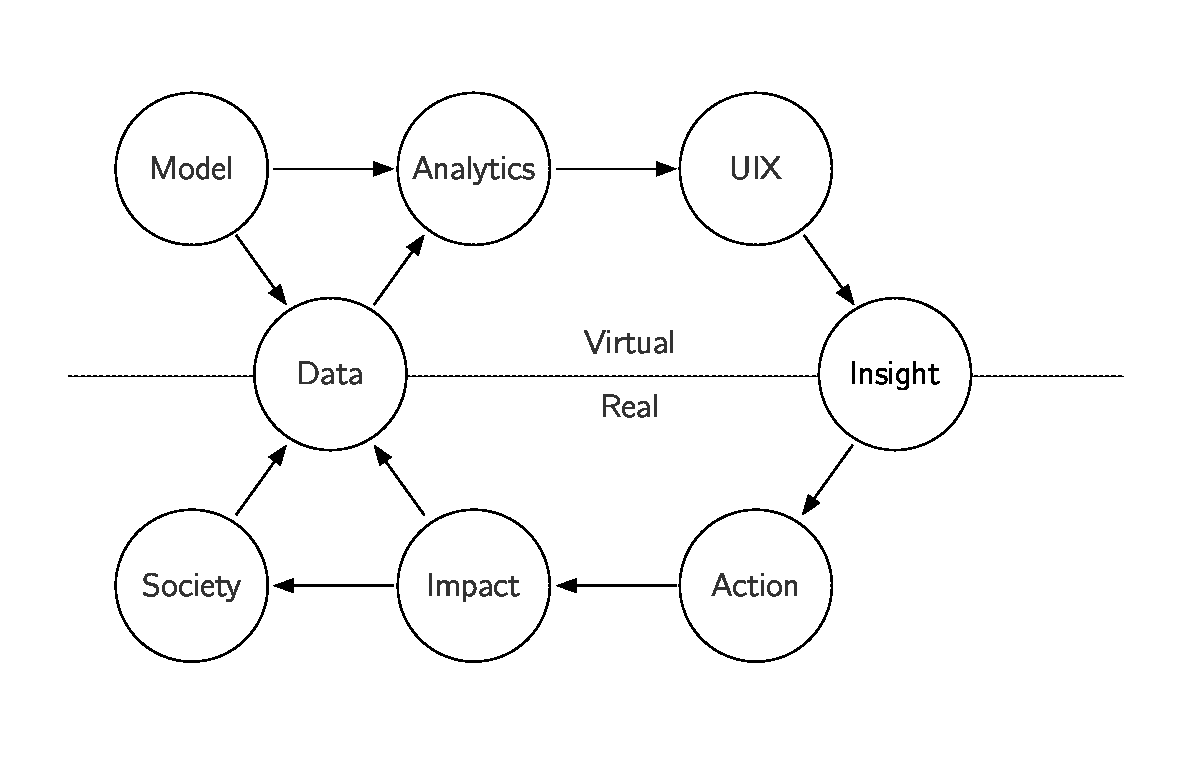
\includegraphics[width=0.8\linewidth]{figures/Loop2.pdf}
    \caption{Sociotechnical system model \cite{winderLoop}}
    \label{fig:loop2}
\end{figure}

In a talk given by Ira \cite{winderLoop}, he describes the paradigm of generating insight from data, which is illustrated in figure \ref{fig:loop2}. He emphesises the role of the user interface, which is essential in getting familiar with the actual data and analytics. The generated insight influences further planning and development. The impact of these actions has the potential to generate new data which feeds back into the loop. The step from data to analytics can be rather intensive and involves creating analytical models. 


\chapter{Existing solutions}
\label{chapter:solutions}
The urban data visualization process can be viewed from multiple perspectives. We can consider the actual physical form of the presentation --- the medium and the the interaction mechanism. On the other hand, it is possible to consider the tools used for the visualization creation, which is more closely related to the standard visualization pipeline. Considering the physical form of the visualization, the examples listed in this chapter can be divided into categories --- purely virtual visualizations, and visualizations with physical components.

\section{Visualization Tools with Physical Components}
This section presents a selected list of visualization tools and projects which use interactive physical components in any shape or form. Due to the nature of these tools, the environment where the visualization is presented plays an important role. It has a profound influence on accessibility, interactivity, and the overall user experience. All presented examples share a common scheme --- a table with interactive physical components is accompanied by a wide-screen projection presenting the actual visualization.   

\paragraph{Tactile Matrix}
Ira Winder and Kent Larson have presented a framework called Tactile Matrix \cite{winderTangible2017}. It is a collaborative tool for real-time computation and projection mapping, see figure \ref{fig:tactilematrix}. The tool is based on a principle described in section \ref{sec:analytics}. The users are presented with a matrix representing city blocks; additional information is conveyed by the visualization projected on top of the matrix. The visualization is driven by an analytical model, which takes the matrix configuration as an input. Lego blocks can be placed into the matrix and the system updates the projection, as the model responds to new inputs. The tool is implemented in Processing, which is a Java-based environment. The SDK for the Tactile Matrix project is available, which also includes the manual to construct the physical components.

\begin{figure}[h]
    \centering
    \begin{subfigure}[t]{0.49\linewidth}
        \centering
        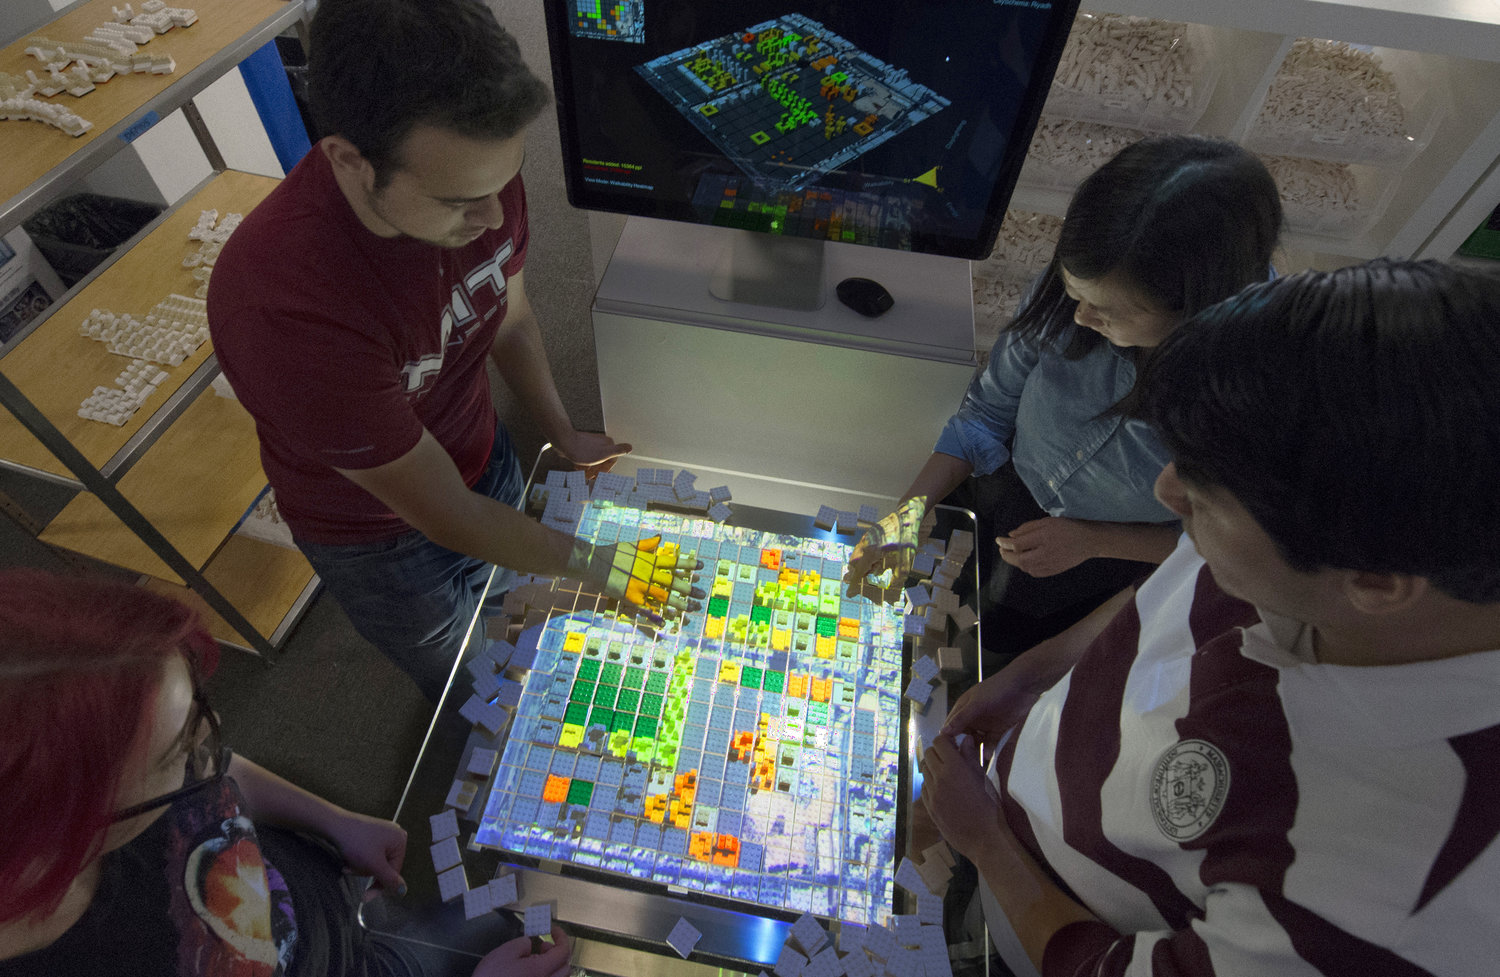
\includegraphics[width=\linewidth]{figures/tactile.jpg}
        \caption{Participants using Tactile Matrix \cite{winderTactileUsers}}
    \end{subfigure}
    \begin{subfigure}[t]{0.49\linewidth}
        \centering
        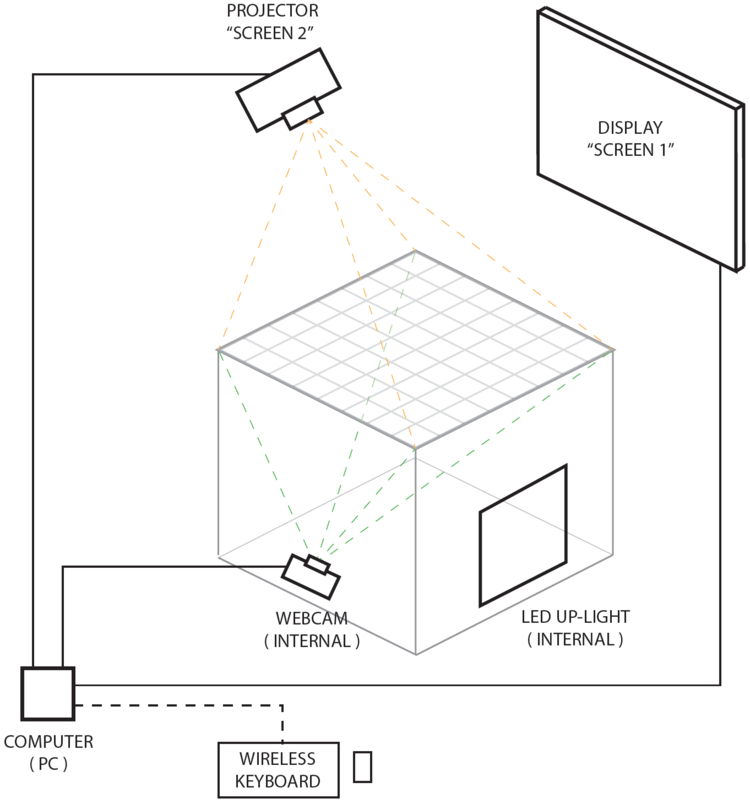
\includegraphics[width=0.6\linewidth]{figures/tactilematrixelectronics.png}
        \caption{SDK Scheme \cite{winderTactileScheme}}
    \end{subfigure}
    \caption{Tactile Matrix framework}
    \label{fig:tactilematrix}
\end{figure}

\paragraph{Pře(d)stav si Prahu} 
In 2019, the OFICINA studio created for IPR Prague an interactive exhibition \cite{oficinaPredstav}. The exhibition aimed to present Strategic Plan for Prague \cite{pragueStrategicPlan}. The visitors had the opportunity to try the role of city planners. The exhibition used the space of the Center for Architecture and Metropolitan Planning (CAMP). The dominant feature of the exhibition was the wide-screen projection displaying the current state of the simulation, see figure \ref{fig:oficinaexhib}. The task of the visitors was to regulate the city life (e.g. tourism, transport), and set the course of the future development (e.g. investments, housing). The simulation was controlled by the amount of colorful blocks on tables (see figure \ref{fig:oficinablocks}), and by analog pulls. Each analog control was assigned a specific action; placing the block or activating the pull sent a new input to the underlying model. The wide-screen visualization provided the visual feedback. The virtual visual components were implemented using web technologies to provide more flexibility.

\begin{figure}[h]
    \centering
    \begin{subfigure}[t]{0.49\linewidth}
        \centering
        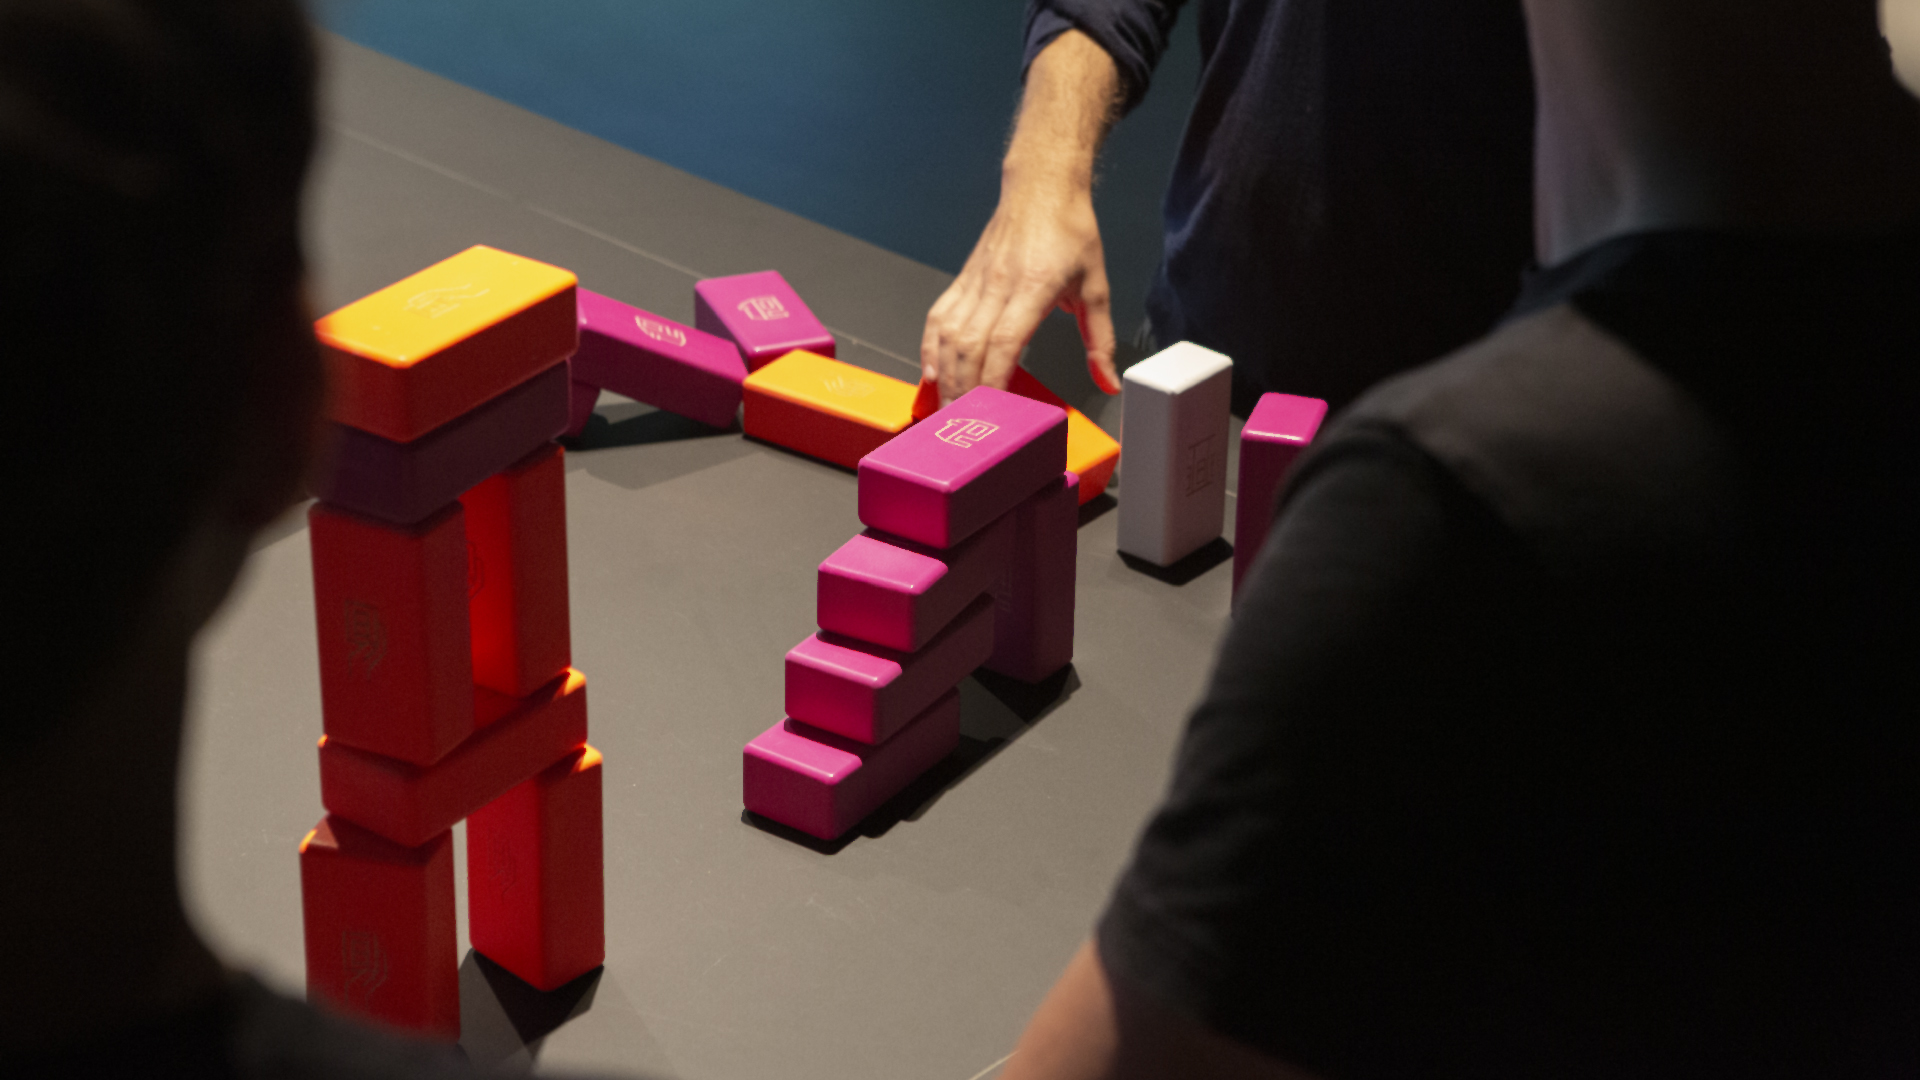
\includegraphics[width=\linewidth]{figures/oficina1.jpg}
        \caption{Color blocks \cite{oficinaPredstav}}
        \label{fig:oficinablocks}
    \end{subfigure}
    \begin{subfigure}[t]{0.49\linewidth}
        \centering
        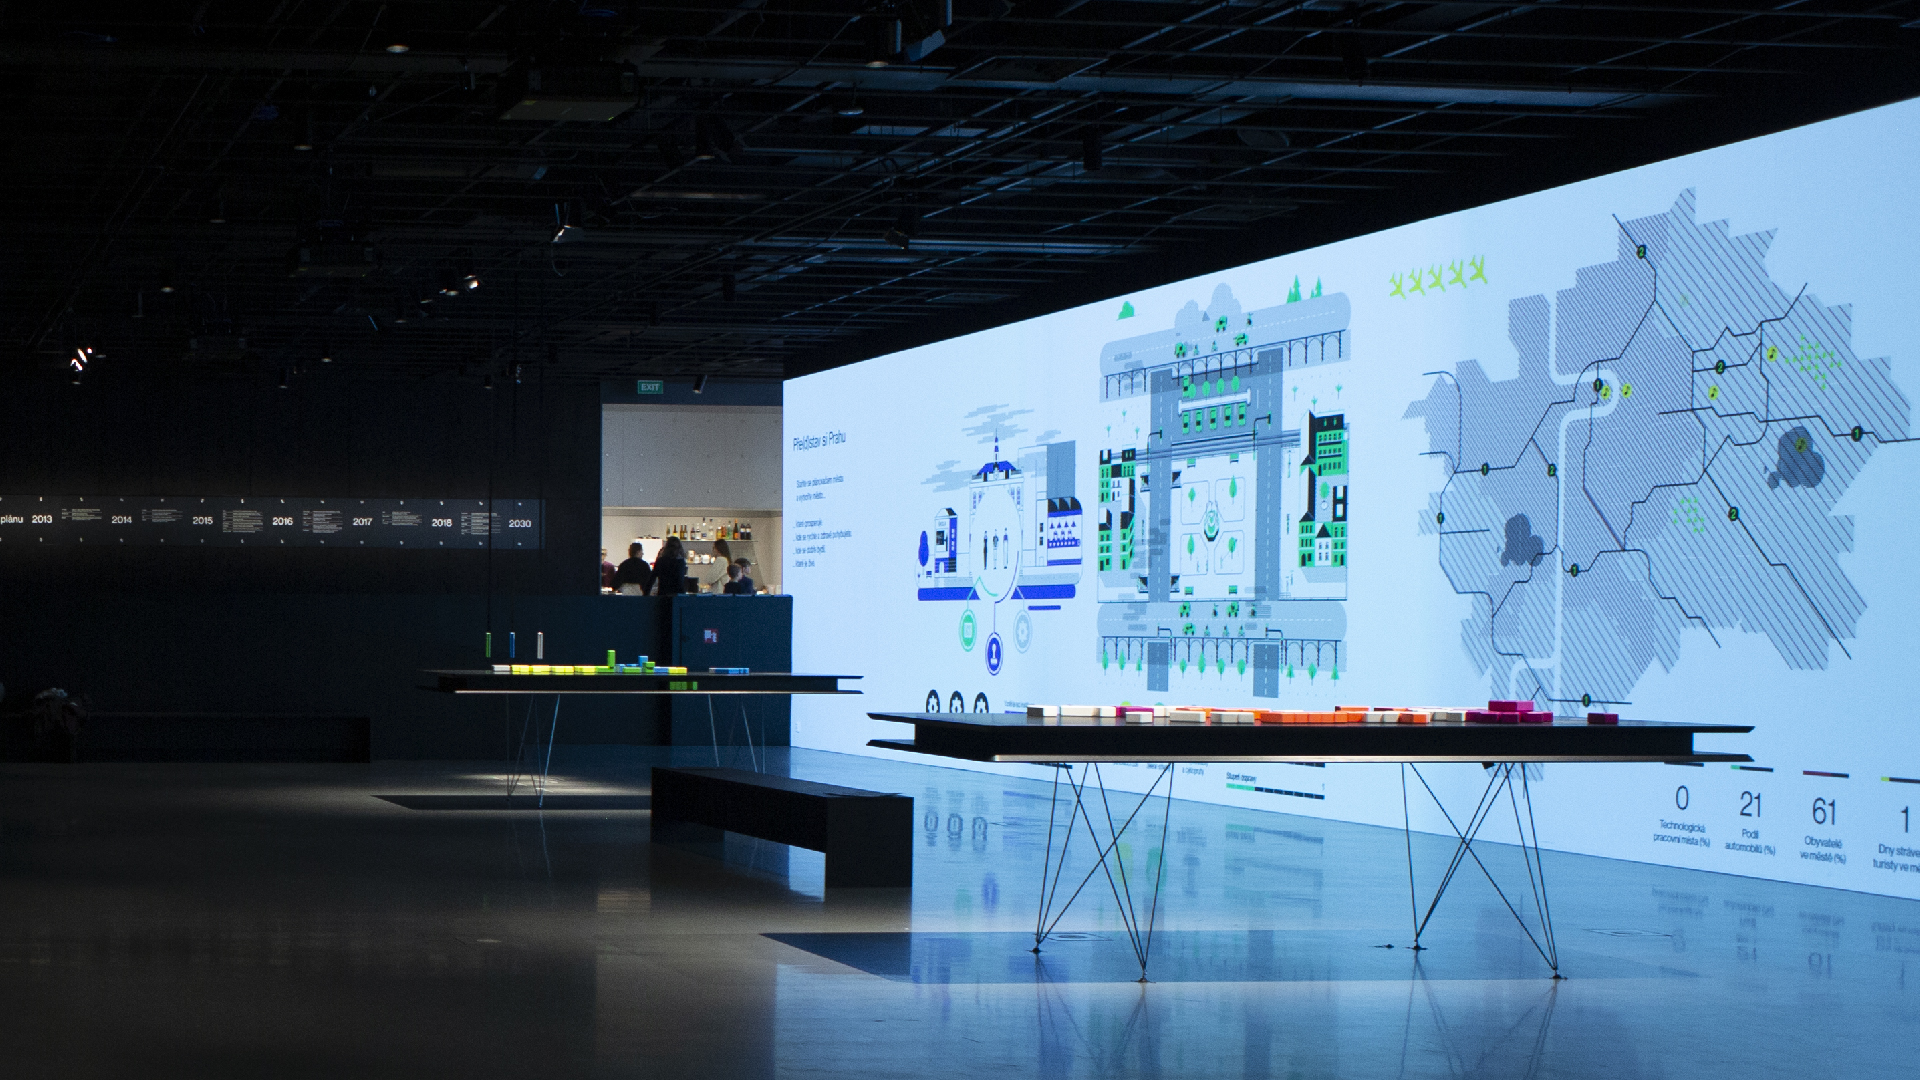
\includegraphics[width=\linewidth]{figures/oficina2.jpg}
        \caption{The exhibition environment \cite{oficinaPredstav}}
        \label{fig:oficinaexhib}
    \end{subfigure}
    \caption{Pře(d)stav si Prahu by OFICINA in CAMP}
    \label{fig:oficinapredstav}
\end{figure}


\paragraph{Rohanský ostrov: nový Karlín?} 
Another exhibition at CAMP in 2019 used a combination of architectural model and projection mapping, more details can be found in \cite{iprRohan}. The exhibition was not interactive; however, the projection served as a visual aid for the visitors standing around the physical model. The projection highlited areas and buildings that will be transformed in the next 20 years.

\begin{figure}[h]
    \centering
    \begin{subfigure}[t]{0.49\linewidth}
        \centering
        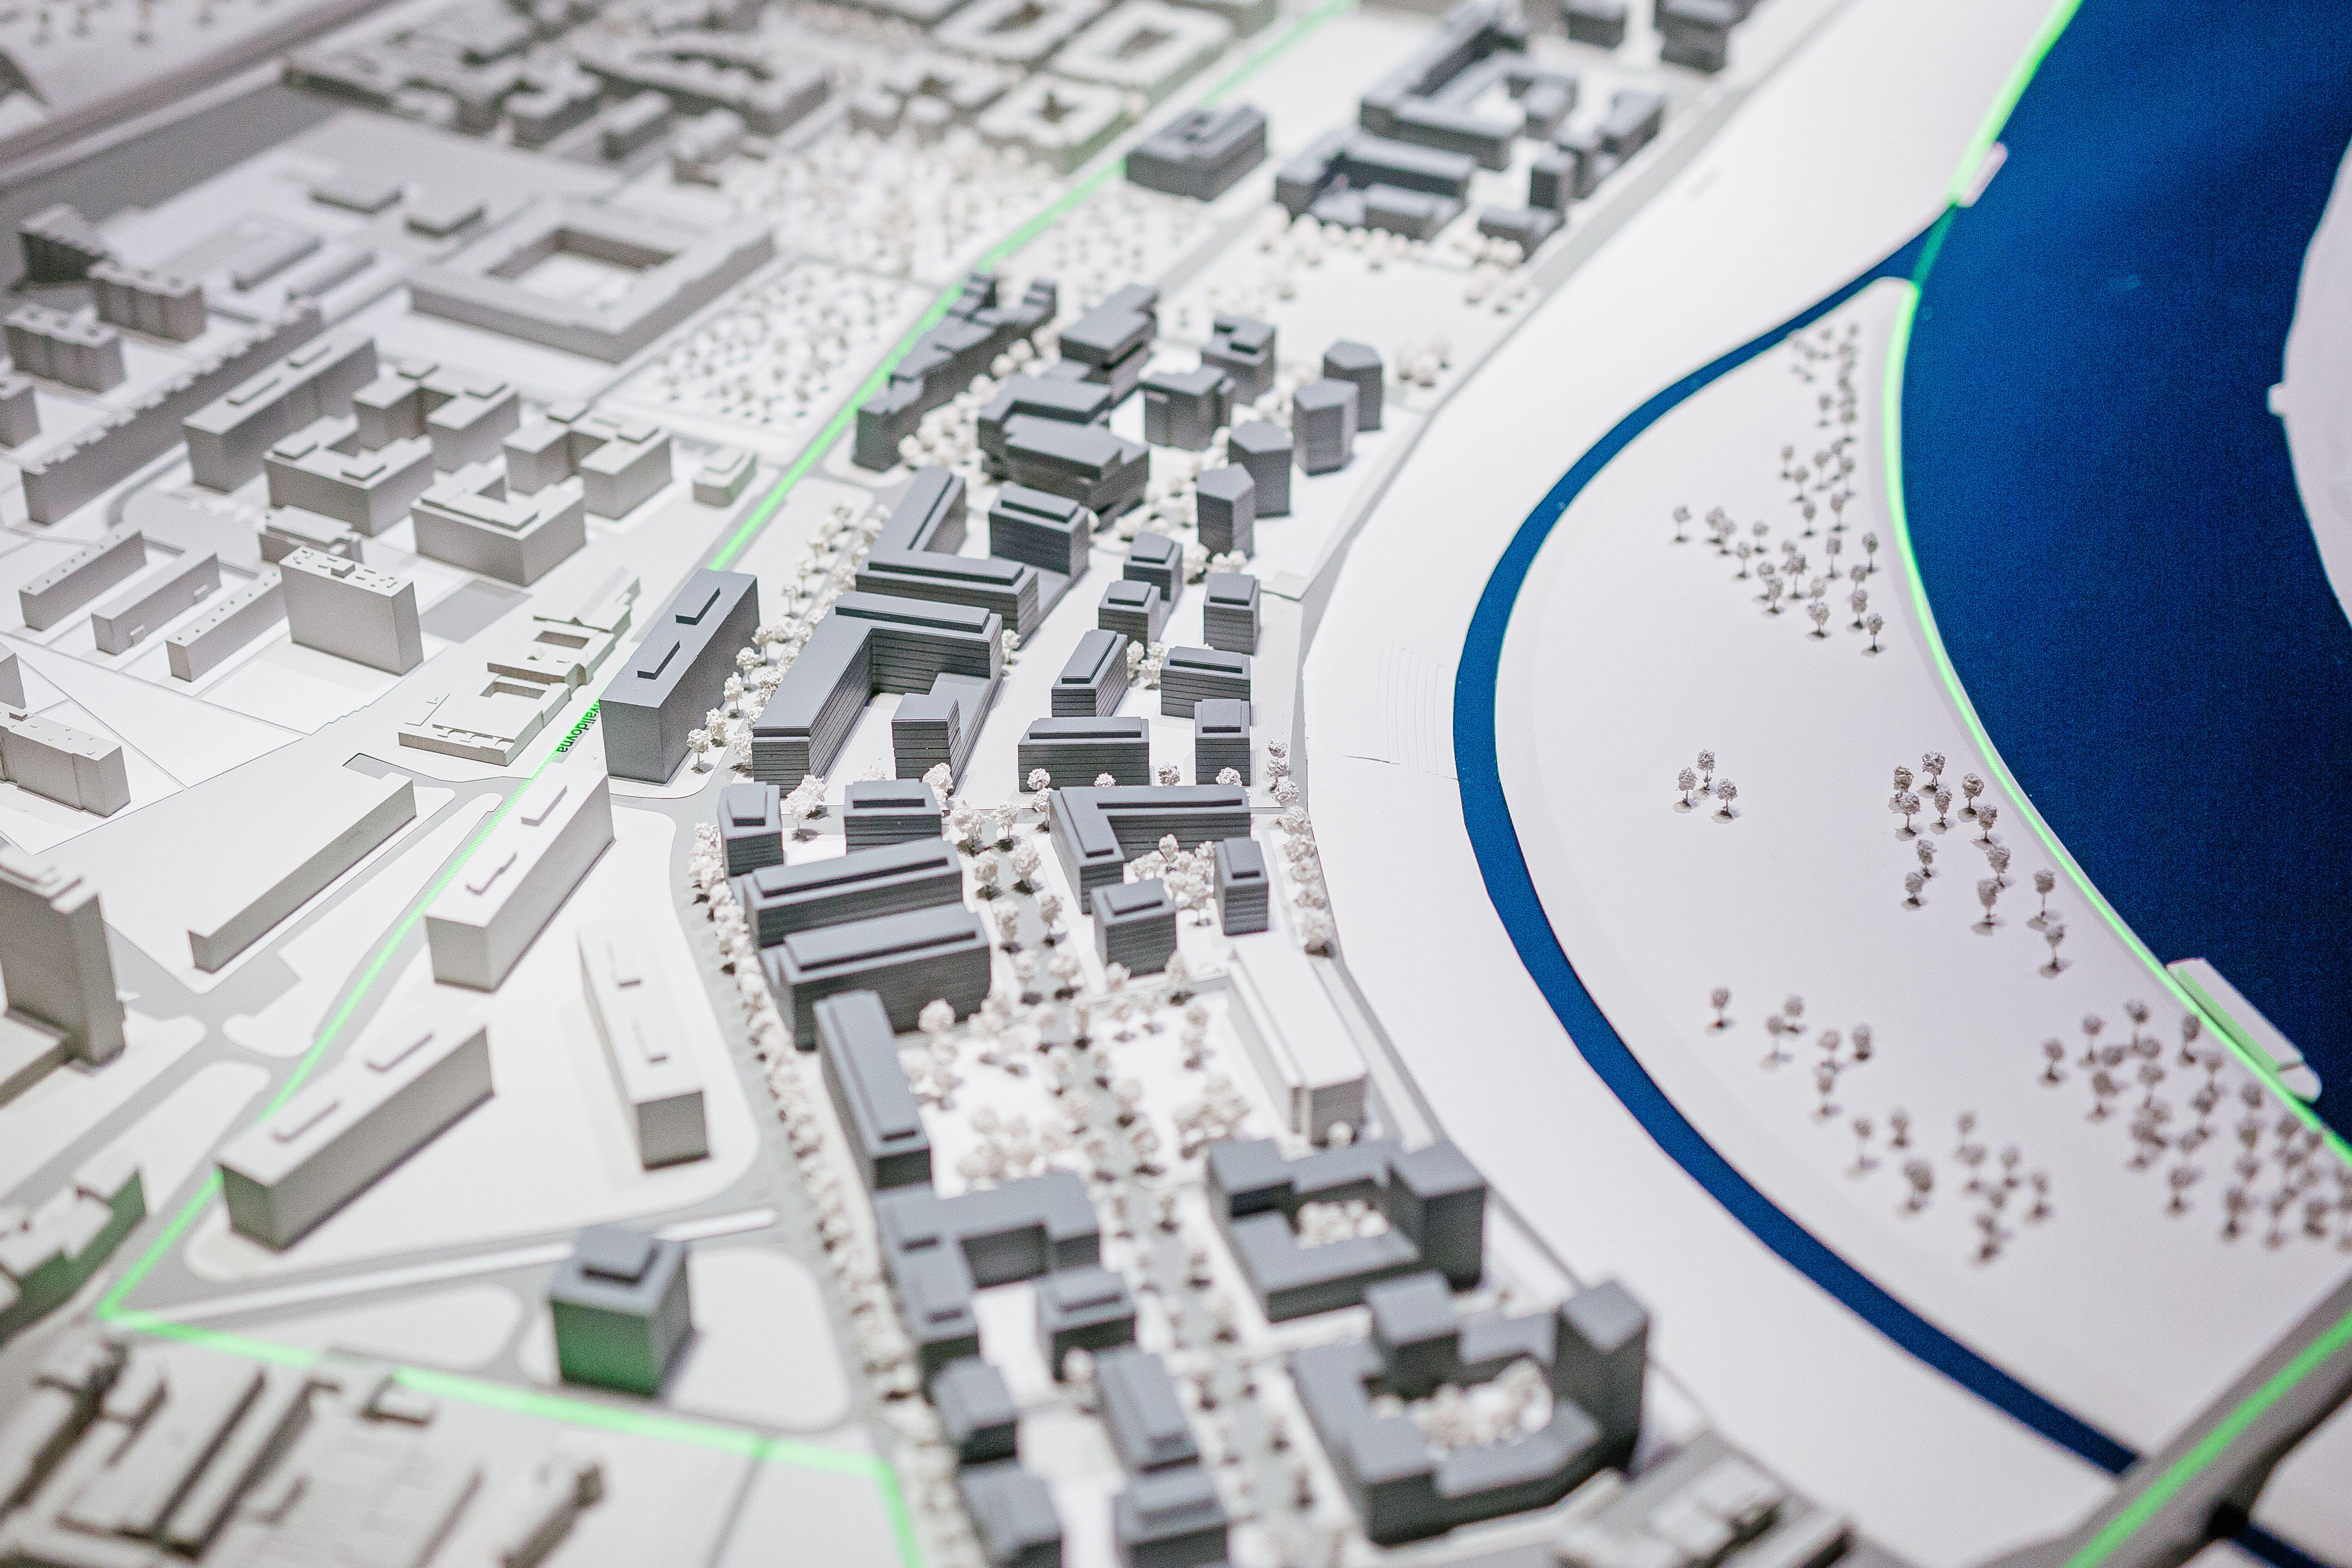
\includegraphics[width=\linewidth]{figures/rohan1.jpg}
        \caption{Highlited area \cite{iprRohanImages}}
        \label{fig:rohanhighlight}
    \end{subfigure}
    \begin{subfigure}[t]{0.49\linewidth}
        \centering
        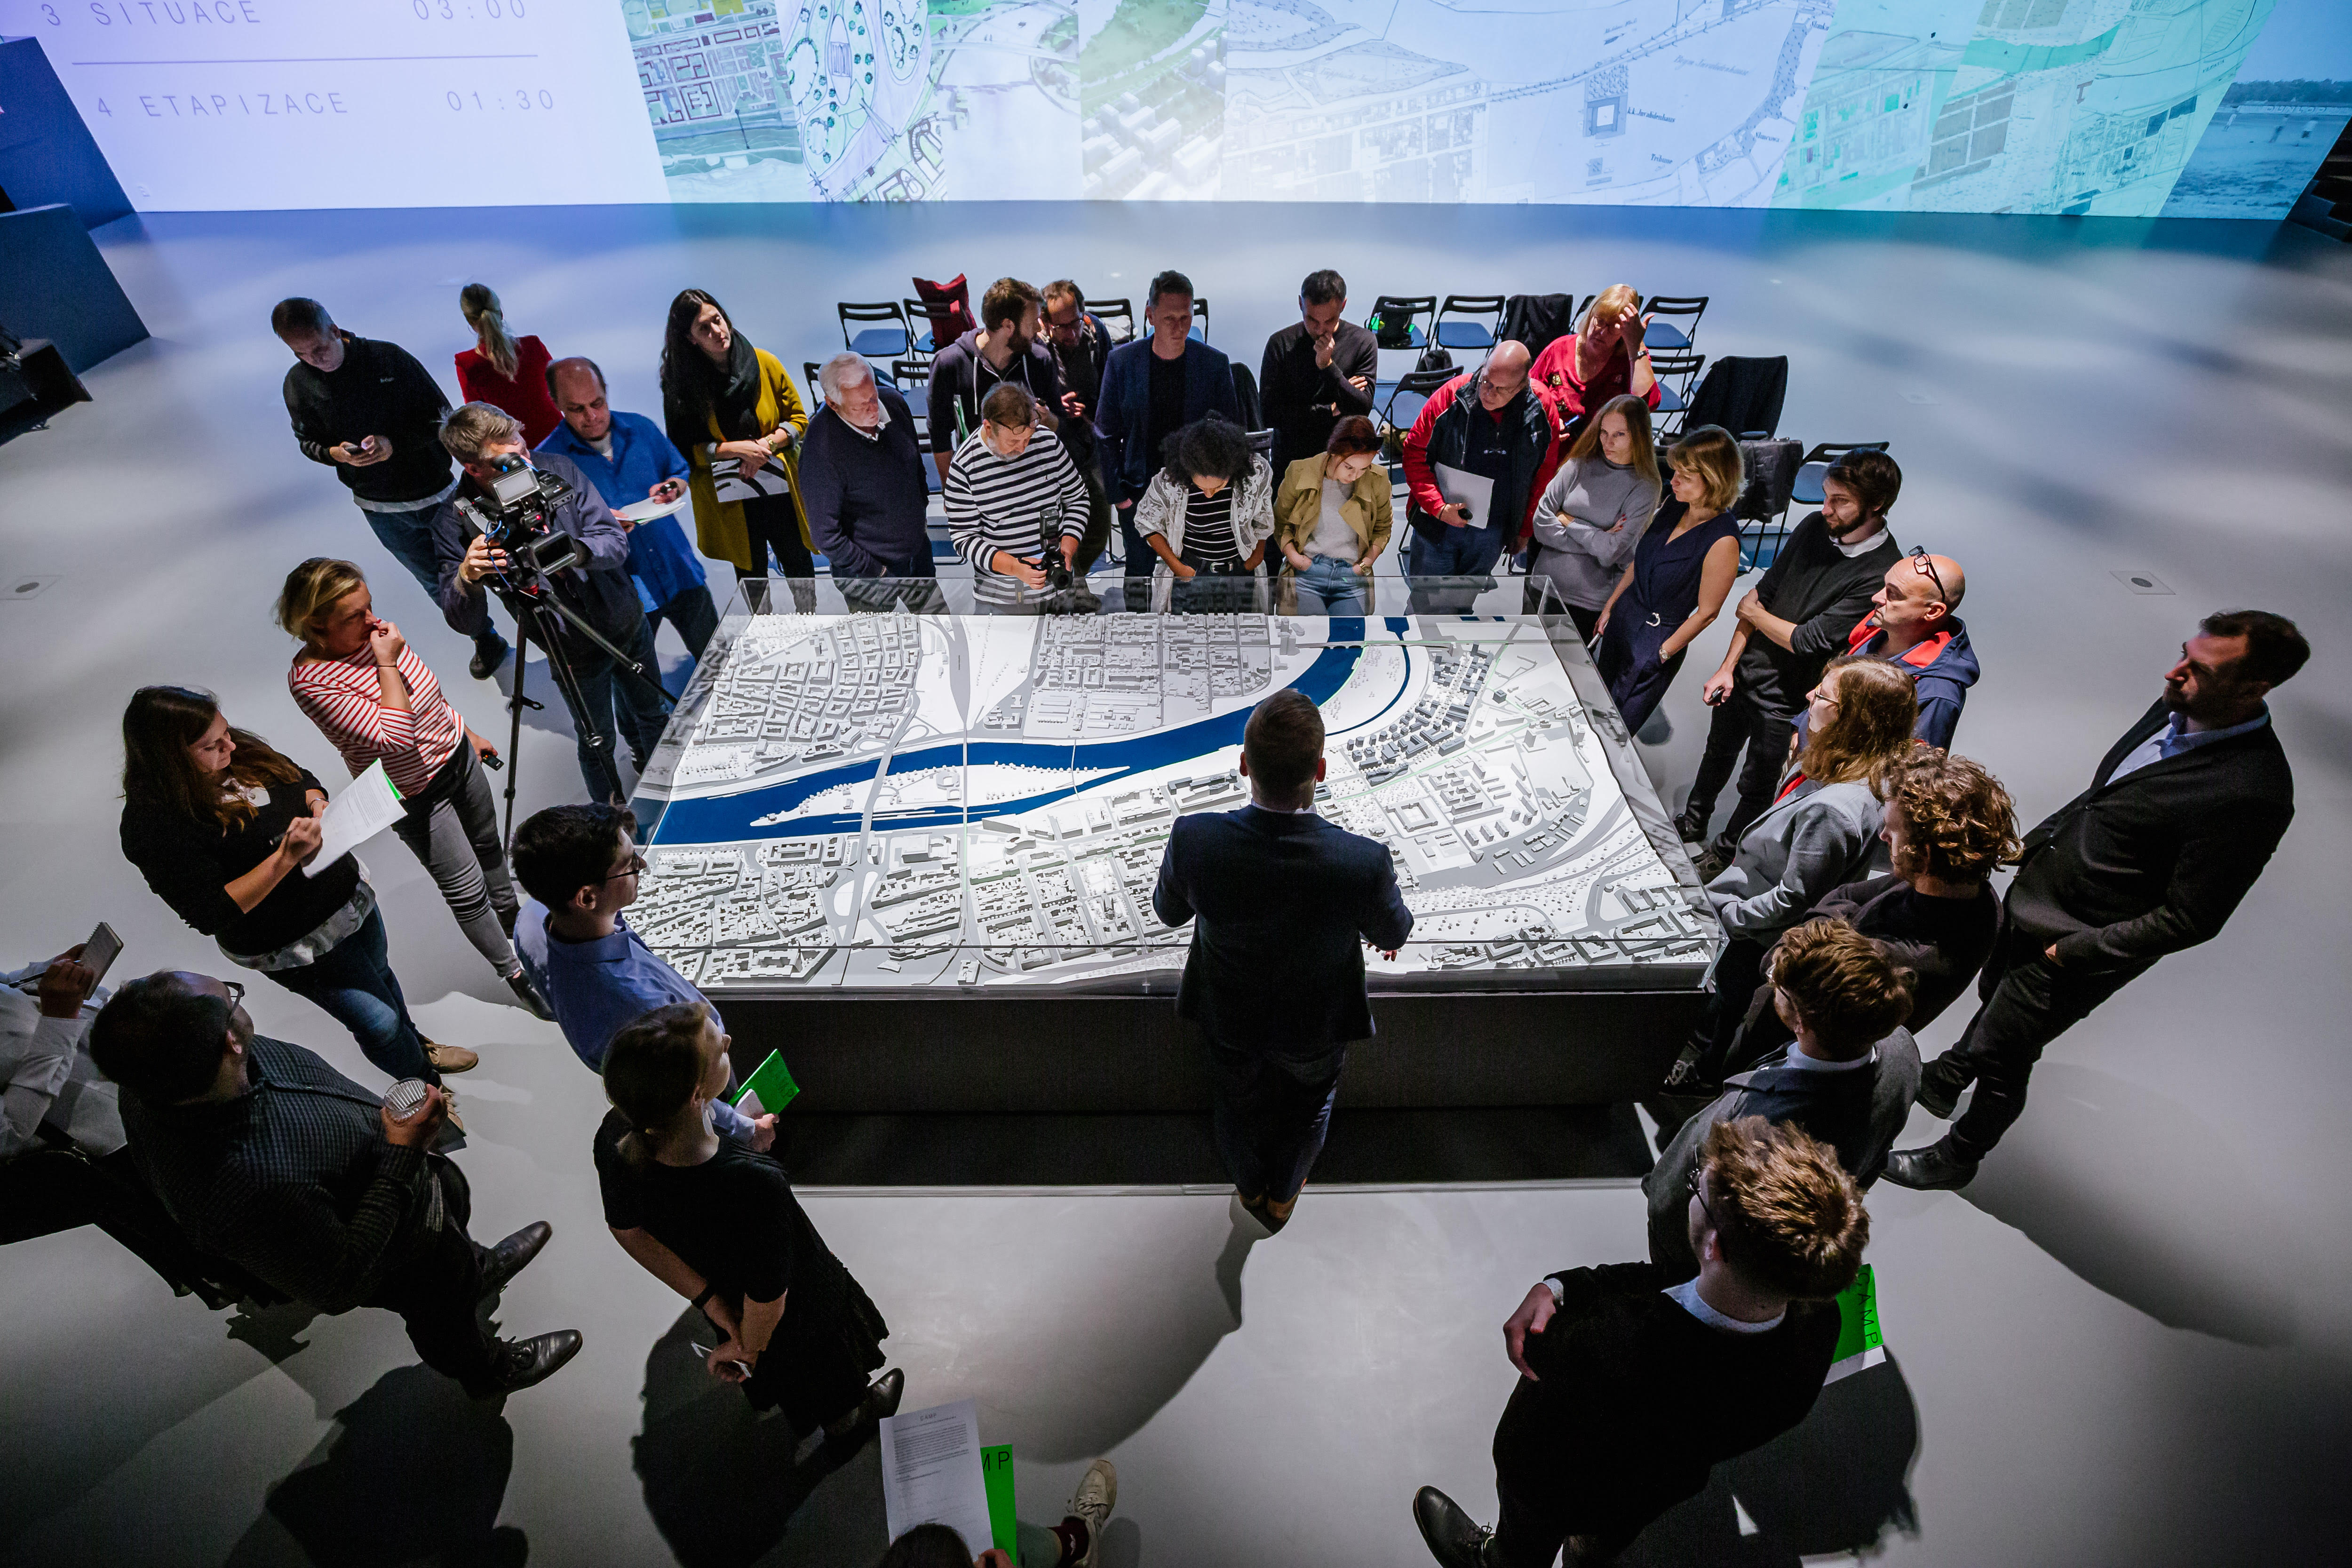
\includegraphics[width=\linewidth]{figures/rohan3.jpg}
        \caption{Physical model \cite{iprRohanImages}}
        \label{fig:rohanmodel}
    \end{subfigure}
    \caption{Rohanský ostrov: nový Karlín? in CAMP}
    \label{fig:rohan}
\end{figure}


\section{Purely Virtual Visualization Tools}
Purely virtual visualization tools are usually a variation of geographic information system (ArcGis, QGIS), but there are a few notable exceptions (kepler.gl, Movement). 

\subsection{Applications}
This section presents the available geospatial visualization applications. As is evidenced by the following list of available applications, the dominant trend in geographic visualization is to move the presentation to the web environment. That has a few advantages:
\begin{itemize}
    \item no need to install any desktop applications
    \item multiplatform apps by default
    \item easily sharable content (it is already on the web)
\end{itemize}

\paragraph{ArcGis} 
Esri offers a range of GIS products under the name of ArcGIS \cite{esriArcgis}. It is a full suite of software for geospatial visualization and analysis. ArcGIS Urban focuses on urban data, visualization, and planning. It is a web-based application. As it is commercial software with full-time support, it is a widely popular solution used by local authorities. ArcGis supports a wide range of proprietary formats (namely ArcIMS, DGN, DWG, DXF, and a range of raster formats). 

\paragraph{QGIS} An open-source alternative to ArcGIS is QGIS \cite{QGISsoftware} --- a tool for creating, viewing, and editing geospatial information. It supports a wide range of formats (Esri Shapefiles, ArcInfo files, MapInfo files, .csv, OpenStreetMap data, PostGis data together with a group of database-based file formats). There is a QGIS plugin, Qgis2threejs, which provides a way to view 3D content in browser, but it appears that the only supported input format is .hgt - DEM (Digital elevation model) format. From version 3.0, there is built-in support for 3D content; supported formats are mostly Esri Shapefiles and raster formats (e.g. GeoTiff). It is possible to export static images as well as short animations created from time-series data. The current capabilities of the program do not allow to customize the styling of the outputs. 

\paragraph{kepler.gl}
Kepler.gl \cite{uberKepler} is an open-source visualization application developed by vis.gl \cite{visgl}. The tool was created and popularized in collaboration with Uber; the main focus is scalability and good performance. The tool is based on Deck.gl, also made by vis.gl, a WebGL-based rendering framework optimized for big data visualizations. The application uses a concept of layers and filters for displaying the imported data. Each layer is an isolated entity with its own base geometry (lines, arcs, points, hex or rectangular grid, heatmap, etc.) and style. 
The application uses OpenStreetMap \cite{openstreetmap} and Mapbox \cite{mapbox} data as a source for 2D maps and 3D models of buildings. The only missing 3D component is the terrain height. It is possible to use Kepler.gl as a Python library for visualization inside Jupyter Notebooks. The supported formats include CSV, GeoJSON, and proprietary JSON-based application format. 

\paragraph{Movement}
This application was also developed by vis.gl in collaboration with Uber \cite{uberMovement}. The primary focus of this application is the visualization of transport-related data. This project stands on the border of visualization and data analysis. Unlike the previous examples, this application was developed to present a fixed set of curated datasets. The goal is to help cities (they operate only in a limited number of cities) to reduce congestion, emissions, and improve road safety.

\paragraph{Cesium}
Cesium \cite{ce2019cesiumjs} is a platform for building geospatial applications. It provides a way to push 3D content to both web (CesiumJS) and Unreal Engine. A part of the services is a platform called Ion, which automatically tiles and optimizes the content for both web and the game engine and offers a library of assets such as images, terrain, and building models. Cesium offers a free plan with a limited amount of data. However, the platform is targeted towards commercial projects and offers pre-paid plans with higher bandwidth.

\subsection{Frameworks}
\label{sec:frameworks}
In terms of visualization frameworks, there are several existing solutions. There is a slight difference between the previous examples and these frameworks --- the frameworks are not standalone visualization solutions. The visualization frameworks usually provide a set of features (data management, rendering, etc.) used throughout the visualization pipeline. 

\paragraph{3DCityDB}
3DCityDB \cite{yao20183dcitydb} is a framework oriented towards effective storing, analysis, and export of the urban data. Part of the toolkit is also a visualization client, but the framework is mainly oriented towards data management. The idea behind this framework is the use of the CityGML standard as the base scheme for the data representation. The framework supports export into several formats, such as Collada, glTF, and KML.

\paragraph{Vis.gl Frameworks}
Vis.gl \cite{visgl} develops several web-based frameworks for visualization. Deck.gl is a WebGL-based rendering framework for visual exploratory data analysis of large geospatial datasets. It's built to be compatible with React (app flow and UI) and Mapbox (source of the base map). A more general-purpose visualization framework is Luma.gl, also a WebGL-based toolkit. To provide a way for plotting various data in 2D, vis.gl developed a library React-vis. As the name already suggests, it is built to be compatible with the React app model.

\paragraph{Blender GIS and Up3date}
Several plugins allow for the import of GIS data into Blender, namely Blender GIS \cite{blendergis} or Up3date \cite{up3date}, which are both still maintained. The supported files include CityJSON, Shapefile vector, raster image, GeoTIFF DEM, OpenStreetMap. 




\appendix

\printindex

\appendix

\bibliographystyle{iso690}
\bibliography{DP_bibliography}

%Zadani
%\ctutemplate{specification.as.chapter}

\end{document}